\documentclass[10pt,a4paper]{article}

% ── Encoding & fonts ──────────────────────────────────────────────────────────
\usepackage[utf8]{inputenc}
\usepackage[T1]{fontenc}

% ── Math ──────────────────────────────────────────────────────────────────────
\usepackage{amsmath}
\usepackage{amsfonts}
\usepackage{amssymb}

% ── Graphics & color ──────────────────────────────────────────────────────────
\usepackage{graphicx}
\usepackage{tikz}
\usetikzlibrary{arrows.meta, positioning, shapes.geometric, fit, calc}

% ── Tables ────────────────────────────────────────────────────────────────────
\usepackage{booktabs}
\usepackage{tabularx}
\usepackage{array}
\usepackage{longtable}
\usepackage{multirow}

% ── Layout ────────────────────────────────────────────────────────────────────
\usepackage[margin=2.5cm]{geometry}
\usepackage{setspace}
\setstretch{1.15}
\usepackage{parskip}

% ── References & links ────────────────────────────────────────────────────────
\usepackage[numbers,sort&compress]{natbib}
\usepackage[hidelinks,
            pdftitle={Triangulation nach Schult},
            pdfauthor={Denis Schult},
            pdfkeywords={LLM, epistemic divergence, multi-agent, triangulation,
                         falsification, labour market, AI methodology}]{hyperref}

% ── Misc ──────────────────────────────────────────────────────────────────────
\usepackage{xcolor}
\usepackage{enumitem}
\usepackage{footnote}
\usepackage{caption}

% ── Metadata ──────────────────────────────────────────────────────────────────
\title{\textbf{Triangulation nach Schult (TNS):}\\
       A Structured Multi-Agent Protocol for\\
       Epistemic Divergence Analysis Using\\
       Large Language Models}

\author{Denis Schult\\
        Independent Researcher, Germany\\
        \texttt{schltdns@gmail.com}\\[0.5em]
        \small Version 1.2-Open \quad April 2026}

\date{}

% ══════════════════════════════════════════════════════════════════════════════
\begin{document}

\maketitle

% ── Abstract ──────────────────────────────────────────────────────────────────
\begin{abstract}
\noindent\textbf{Background.}
Large Language Models (LLMs) frequently converge due to shared training data,
alignment constraints, and similar optimization objectives.
This convergence can mask systematic errors when multiple models confidently agree
on incorrect or incomplete assumptions.

\noindent\textbf{Objective.}
We introduce \textit{Triangulation nach Schult} (TNS), a structured, prompt-level
multi-agent protocol that treats divergence—contradiction, refusal, and
normative disagreement—as an epistemic signal rather than noise.

\noindent\textbf{Method.}
The protocol comprises eight phases (P1–P8): hypothesis formulation with
falsification thresholds, role-based model selection, parallel elicitation,
divergence mapping and typing, weighted human synthesis, external validation,
operator reflection, and versioned archiving.
Divergence is classified along four axes: substantive, normative, didactic, and
architectural.
A power layer (P6b) provides a meta-filter asking who controls the technology,
who has access, who profits, and who bears the risks.

\noindent\textbf{Results.}
Two documented case studies demonstrate feasibility and scalability.
Case Study~1 (European gas market, three models, April 2026) reveals how a
model refusal can be treated as a productive underspecification signal.
Case Study~2 (German labour market 2030, six models—ChatGPT, Claude, DeepSeek,
Gemini, Grok, Copilot) produces a divergence-structured synthesis across seven
analytical dimensions (A–G), including testable falsification criteria with explicit
thresholds (e.g., EU productivity growth $<0.1\%$~p.a.\ by 2028 would falsify the
optimistic productivity thesis) and a power-layer audit of each core claim.

\noindent\textbf{Conclusion.}
TNS is a heuristic, human-centered framework for reflective decision-making under
uncertainty. It is suitable for didactic, analytical, and policy contexts. Limitations
include dependence on operator judgment and sensitivity to model drift.
The protocol and both case studies are openly available at
\url{https://github.com/schltdns}.

\bigskip
\noindent\textbf{Keywords:} large language models; multi-agent systems; epistemic
divergence; falsification; triangulation; labour market; AI methodology; human-in-the-loop
\end{abstract}

\tableofcontents
\newpage

% ══════════════════════════════════════════════════════════════════════════════
\section{Introduction}
\label{sec:intro}

Large Language Models have moved from niche research tools to widely deployed
decision-support systems. Their tendency to produce confident, fluent, and plausible
outputs raises a fundamental epistemic problem: when multiple models agree,
this agreement does not constitute evidence of correctness. Shared training corpora,
common fine-tuning objectives, and similar alignment procedures mean that divergence
between models is comparatively rare—and therefore informative when it occurs
\citep{denzin1970,Liang2024}.

Existing approaches to multi-model integration—ensemble methods, debate
frameworks, red teaming—typically aim either to improve aggregate accuracy or to
stress-test a single model \citep{Du2023,Perez2022}. Neither paradigm treats
persistent divergence as a primary research signal.

\textit{Triangulation nach Schult} (TNS)\footnote{The term ``triangulation''
is used in the sociological tradition of \citet{denzin1970} and
\citet{patton1999}, where multiple data sources are used not to confirm but to
reveal discrepancies. TNS extends this logic to LLM outputs.}
addresses this gap. Rather than forcing convergence, the protocol maps, classifies,
and interprets divergence as a proxy for structural uncertainty. The human operator
is positioned not as a passive recipient of model outputs but as an active
integrator who must justify every synthesis decision.

This paper makes the following contributions:
\begin{enumerate}[leftmargin=*, label=(\arabic*)]
  \item A complete, phase-by-phase protocol (P1–P8) with explicit falsification
        rules and operator obligations.
  \item A four-axis divergence typology (substantive, normative, didactic,
        architectural) that distinguishes resolvable from irreducible disagreement.
  \item A power layer (P6b) as a fourth meta-filter, extending the protocol beyond
        epistemics into questions of access, control, and distribution.
  \item Two documented case studies of different scale and complexity,
        demonstrating feasibility and scalability.
\end{enumerate}

% ══════════════════════════════════════════════════════════════════════════════
\section{Related Work}
\label{sec:related}

\subsection{Delphi Method}
\citet{dalkey1963} developed iterative expert elicitation aiming for consensus.
TNS differs by foregrounding divergence rather than reducing it, and by using LLMs
as investigator proxies rather than human experts.

\subsection{Ensemble Methods in Machine Learning}
Ensemble approaches combine model outputs to improve predictive accuracy
\citep{breiman1996}. They optimize for agreement; TNS optimizes for structured
disagreement as a diagnostic signal.

\subsection{Multi-Agent Debate}
\citet{Du2023} and \citet{Liang2024} demonstrate that LLMs critiquing each other's
outputs can improve factual accuracy. Their protocols aim for resolution; TNS
preserves and documents unresolved divergence.

\subsection{Red Teaming}
\citet{Perez2022} probe single models adversarially to surface vulnerabilities. TNS
uses multiple heterogeneous models simultaneously, comparing their outputs rather
than attacking one.

\subsection{SCOUT and Semantic Triangulation}
Automated uncertainty prediction methods \citep{xiong2024} use statistical
properties of model outputs. TNS is qualitative and role-based, foregrounding
human judgment rather than automated scoring.

\subsection{Multi-Agent Orchestration Frameworks}
Frameworks such as AutoGen \citep{wu2023autogen}, CrewAI, and OpenAI Swarm
solve a technical coordination problem. TNS operates at a higher logical level: it
provides the \textit{epistemic logic} for interpreting disagreement and can be
implemented on top of any framework that supports parallel model queries.
Where orchestration frameworks seek efficiency and task completion, TNS seeks
interpretable divergence.

\subsection{Constructivist Pedagogy}
\citet{reich2008} argues that knowledge construction requires encountering
alternative perspectives that cannot be immediately resolved. TNS operationalizes
this principle in the context of AI-assisted analysis: unresolved divergence is not a
failure state but a productive pedagogical and epistemic resource.

% ══════════════════════════════════════════════════════════════════════════════
\section{The TNS Framework}
\label{sec:framework}

\subsection{Core Principle}
\textbf{Divergence is a signal, not noise.}

The protocol uses multiple LLMs as \textit{perspective generators}. Each model
contributes a distinct epistemic function determined by its architecture, training
data, alignment, and cultural context.

\subsection{Divergence Typology}
\label{sec:typology}

TNS classifies divergence along four axes:

\begin{table}[h]
\centering
\caption{TNS divergence typology with handling rules.}
\label{tab:typology}
\begin{tabularx}{\textwidth}{lXl}
\toprule
\textbf{Type} & \textbf{Definition} & \textbf{Synthesis handling} \\
\midrule
Substantive & Different facts, causal mechanisms, or quantitative estimates & Resolved by external validation; bandwidth if unresolved \\
Normative & Different value priorities, risk tolerances, or policy preferences & Documented as open question; power-layer check \\
Didactic & Different explanation styles or examples with same underlying claim & Ignored in synthesis \\
Architectural & Different model assumptions traceable to training data or alignment & Noted; not arithmetically merged \\
\bottomrule
\end{tabularx}
\end{table}

Only substantive and normative divergence enter the final synthesis with weighting.
Didactic differences are set aside. Architectural differences are documented as
provenance information.

\subsection{The Three-Filter Model}
\label{sec:filters}

For applied case studies, TNS introduces a three-filter model to structure how
divergence maps onto real-world transformation processes:

\begin{enumerate}[leftmargin=*, label=\textbf{Filter \arabic{*}.}]
  \item \textbf{Adoption filter} — Can organisations re-design processes to absorb
        the technology?
  \item \textbf{Qualification filter} — Do individuals have or can acquire the
        skills required?
  \item \textbf{Institution filter} — Do regulatory and educational systems adapt
        quickly enough?
\end{enumerate}

This model operationalizes the \textit{master question} of applied TNS studies:
\textit{Does the technology scale faster than social systems can adapt?}

\subsection{The Power Layer (P6b)}
\label{sec:powerlayer}

The three filters are not power-neutral. For every core synthesis claim, TNS requires
a power-layer check addressing four questions:
\begin{enumerate}[leftmargin=*, label=(\arabic*)]
  \item Who controls the technology?
  \item Who has access to it?
  \item Who profits from its deployment?
  \item Who bears the risks of its failure or misuse?
\end{enumerate}

The power layer is a \textit{meta-filter}: it applies on top of all three filters and
all synthesis conclusions. Without it, the analysis remains technocratic—accurate
about what technology can do but blind to for whom and at whose expense.

% ── Protocol diagram ──────────────────────────────────────────────────────────
\subsection{Protocol Overview (P1--P8)}

Figure~\ref{fig:protocol} shows the eight-phase cycle.

\begin{figure}[h]
\centering
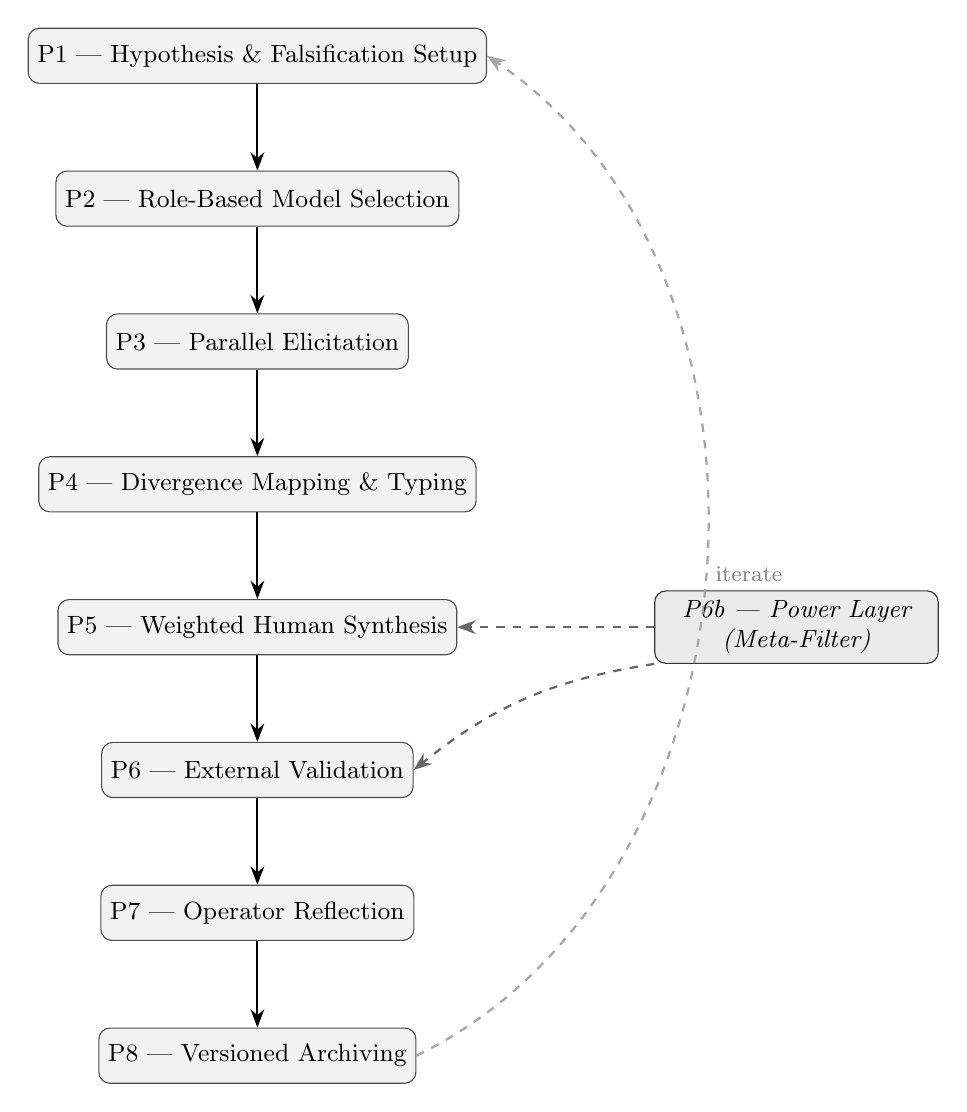
\begin{tikzpicture}[
  node distance = 1.1cm and 2.2cm,
  box/.style  = {rectangle, rounded corners=4pt, draw=black!70, fill=gray!10,
                 minimum width=3.6cm, minimum height=0.7cm,
                 font=\small, align=center},
  powerbox/.style = {rectangle, rounded corners=4pt, draw=black!80,
                     fill=black!8, minimum width=3.6cm, minimum height=0.7cm,
                     font=\small\itshape, align=center},
  arr/.style  = {-Stealth, thick},
  every node/.style = {font=\small}
]

\node[box] (p1) {P1 — Hypothesis \& Falsification Setup};
\node[box, below=of p1] (p2) {P2 — Role-Based Model Selection};
\node[box, below=of p2] (p3) {P3 — Parallel Elicitation};
\node[box, below=of p3] (p4) {P4 — Divergence Mapping \& Typing};
\node[box, below=of p4] (p5) {P5 — Weighted Human Synthesis};
\node[powerbox, right=2.5cm of p5] (pl) {P6b — Power Layer\\(Meta-Filter)};
\node[box, below=of p5] (p6) {P6 — External Validation};
\node[box, below=of p6] (p7) {P7 — Operator Reflection};
\node[box, below=of p7] (p8) {P8 — Versioned Archiving};

\draw[arr] (p1) -- (p2);
\draw[arr] (p2) -- (p3);
\draw[arr] (p3) -- (p4);
\draw[arr] (p4) -- (p5);
\draw[arr] (p5) -- (p6);
\draw[arr] (p6) -- (p7);
\draw[arr] (p7) -- (p8);
\draw[arr, dashed, draw=black!60] (pl.west) -- (p5.east);
\draw[arr, dashed, draw=black!60] (pl.south west) to[bend right=15] (p6.east);

% Feedback arrow
\draw[arr, draw=gray!70, dashed]
  (p8.east) to[bend right=60] node[right, font=\footnotesize, text=gray]
  {iterate} (p1.east);

\end{tikzpicture}
\caption{The eight-phase TNS cycle. Dashed arrows indicate the power-layer
meta-filter (P6b) applied during synthesis and validation. The feedback loop
from P8 back to P1 supports iterative refinement.}
\label{fig:protocol}
\end{figure}

% ══════════════════════════════════════════════════════════════════════════════
\section{The Eight-Phase Protocol (P1--P8)}
\label{sec:protocol}

\subsection{P1 — Hypothesis and Falsification Setup}
Define one or more hypotheses with explicit falsification thresholds before
eliciting model responses.
Example: \textit{H1 is rejected if EU productivity growth remains below
$0.1\%$~p.a.\ through 2028.}
Pre-registration of falsification criteria prevents post-hoc rationalization.

\subsection{P2 — Role-Based Model Selection}
Assign available models to functional roles. Roles are descriptive, not prescriptive.

\begin{table}[h]
\centering
\caption{Illustrative functional role mapping.}
\label{tab:roles}
\begin{tabular}{ll}
\toprule
\textbf{Role} & \textbf{Function} \\
\midrule
Structural model  & Logical framing, decomposition \\
Boundary model    & Normative constraints, safety logic \\
Adversarial model & Stress-testing, contradiction exposure \\
Didactic model    & Process reflection, explanation \\
Synthesis model   & Operational integration \\
Human operator    & Judgment, prioritization, meta-reflection \\
\bottomrule
\end{tabular}
\end{table}

\subsection{P3 — Parallel Elicitation}
All models receive an identical prompt. Prompt constancy ensures that divergence
reflects model differences, not query differences.

\subsection{P4 — Divergence Mapping and Typing}
Contradictions are classified using the typology in Table~\ref{tab:typology}.
A divergence log records: the dimension, the model positions, the type, and the
relevance for synthesis.

\subsection{P5 — Weighted Human Synthesis}
The human operator integrates perspectives and must justify every deviation from
a model's argument. The synthesis is invalid if the operator cannot articulate why
a model's position was discounted (see P7).

\subsection{P5b / P6b — Power Layer Application}
For every core synthesis claim, the four power questions (Section~\ref{sec:powerlayer})
are applied. Answers are documented; where unknown, the gap is recorded as a
limitation.

\subsection{P6 — External Validation}
Core claims are checked against independent empirical sources at three levels:
(1)~fact-level (do numbers match?),
(2)~causality-level (is the mechanism supported?),
(3)~robustness-level (does the claim hold under alternative assumptions?).
Claims contradicted by validation sources are discarded or downgraded to
``plausible but unconfirmed.''

\subsection{P7 — Operator Reflection}
Three guiding questions:
\begin{enumerate}[leftmargin=*, label=(\arabic*)]
  \item Which perspective dominated the synthesis — and why?
  \item Which perspective was ignored — and can that be justified?
  \item Which assumption remained unfalsified, and what evidence would falsify it?
\end{enumerate}
The operator documents known biases (e.g., regional focus, recency bias) and the
conditions under which their weighting decisions would be falsified.

\subsection{P8 — Versioned Archiving}
The complete artefact — prompts, raw responses, divergence log, synthesis, and
operator reflection — is committed to a version-controlled repository. Every
substantive update to the synthesis triggers a new version number. This
operationalizes \citet{popper1959}: claims must be revisable in light of new evidence.

% ══════════════════════════════════════════════════════════════════════════════
\section{Falsification Rules}
\label{sec:falsrules}

\paragraph{Rule~1 — Iterative Divergence Rule.}
If after $N=3$ parallel elicitations the divergence pattern remains structurally
identical (same contradiction class, same models), the hypothesis is marked
\textit{inconclusive} rather than falsified.

\paragraph{Rule~2 — Refusal Rule.}
If a model refuses with generic safety language, a substitute model is used.
If two substitutes also refuse, the hypothesis is marked \textit{underspecified}
and returned to P1 for reformulation.

\paragraph{Rule~3 — Human Justification Rule.}
If the operator cannot justify ignoring a model's argument, the synthesis is
\textit{invalid} and must be rerun from P5.

\paragraph{Rule~4 — External Review Rule.}
A human reviewer evaluates the synthesis without knowing which model produced
which output. This controls for authority bias (over-weighting well-known models).

% ══════════════════════════════════════════════════════════════════════════════
\section{Case Study 1: European Gas Market (April 2026)}
\label{sec:cs1}

\subsection{Setup}
A test was conducted on April 4, 2026, using three models (Grok, Claude, Copilot)
with an identical prompt analyzing TTF gas prices and German industrial resilience
during the Hormuz supply-disruption scenario.

\subsection{Findings}
\begin{itemize}
  \item Grok and Claude partially confirmed the core hypotheses about price
        transmission and industrial substitution.
  \item Copilot refused to answer as stated, requesting operational definitions
        for ``industrial resilience.''
  \item The refusal was treated as a \textit{meta-signal} indicating underspecified
        hypotheses rather than model failure—an instance of Falsification Rule~2.
  \item The synthesis produced a coherent provisional assessment: the market is
        driven by a real supply shock with structural industrial adaptation under way.
  \item No falsification rule was triggered; the result is considered
        \textit{non-falsified but provisional}.
\end{itemize}

\subsection{Methodological Observation}
The refusal-as-signal treatment demonstrates a core TNS design choice: model
behaviour that would be discarded in consensus-oriented approaches is here
treated as diagnostic information about hypothesis quality.

% ══════════════════════════════════════════════════════════════════════════════
\section{Case Study 2: German Labour Market 2030}
\label{sec:cs2}

\subsection{Setup and Motivation}
Case Study~2 scales the protocol from three to six models and from a single
analytical question to seven interconnected dimensions. The topic—German labour
market transformation under AI automation—was chosen because it exhibits
precisely the conditions TNS is designed to handle: genuine empirical uncertainty,
strong normative disagreement, and structural power asymmetries.

\textbf{Models:} ChatGPT, Claude, DeepSeek, Gemini, Grok, Copilot.\\
\textbf{Date:} April 6, 2026.\\
\textbf{Prompt:} Identical structured prompt across all models covering dimensions
A–G (see below).\\
\textbf{Synthesis operator:} Denis Schult.\\
\textbf{Validation sources:} IAB \citep{iab2025}, WEF \citep{wef2025},
IW~Köln \citep{iw2025}, McKinsey \citep{mckinsey2024}, BAuA \citep{baua2025}.

\subsection{Analytical Dimensions (A--G)}

\begin{table}[h]
\centering
\caption{Seven analytical dimensions of Case Study 2.}
\label{tab:dims}
\begin{tabularx}{\textwidth}{lX}
\toprule
\textbf{Dim.} & \textbf{Core issues} \\
\midrule
A — Economic      & Productivity gains, net job balance, wage dispersion, high-automation sectors, new job profiles, macroeconomic effects \\
B — Technological & Automation level by sector, agentic systems \& multimodal models, human–machine cooperation vs.\ substitution, skill shift, diffusion speed \\
C — Social        & Social mobility, inequality \& polarisation, age risks (50+), regional differences (urban/rural, East/West, EU/US/Asia), mental health \\
D — Education     & Future of vocational training, upskilling/reskilling, future-proof competencies, AI-supported learning (tutors, simulations, AR/VR), dual training \\
E — Policy        & Working-time models (4-day week), migration as buffer, AI regulation (EU AI Act), welfare-state adjustments (basic income, wage subsidies) \\
F — Corporate     & Re-skilling vs.\ layoffs, AI-driven organisational models, leadership \& management, cost–benefit analysis of automation, work-process change \\
G — Divergence    & Job loss vs.\ job change, speed of automation, role of vocational training, winner/loser sectors, optimistic vs.\ pessimistic scenarios, normative assessments \\
\bottomrule
\end{tabularx}
\end{table}

\subsection{Divergence Matrix}

Table~\ref{tab:divergence} summarises the divergences extracted across all six models.

\begin{table}[h]
\centering
\caption{Divergence matrix — six models, seven dimensions (selected high-relevance items).}
\label{tab:divergence}
\resizebox{\textwidth}{!}{%
\begin{tabular}{llllll}
\toprule
\textbf{Dim.} & \textbf{Topic} & \textbf{Cluster A} & \textbf{Cluster B} & \textbf{Type} & \textbf{Relevance} \\
\midrule
A & Net job balance
  & ChatGPT, Gemini, Copilot: net positive, manageable transitions
  & Claude: positive but hard for 50+; DeepSeek: critical for mid-quals
  & Normative & High \\
B & Speed of automation
  & ChatGPT, Gemini, Copilot: gradual, culture-dependent
  & Claude, DeepSeek: exponential, already visible; Grok: volatile
  & Substantive & High \\
E & EU AI Act
  & ChatGPT, Copilot: balance protection/innovation
  & Claude, DeepSeek: brake on innovation; Gemini: pro-regulation
  & Normative & High \\
D & Dual training
  & ChatGPT, Gemini, Copilot: clear competitive advantage
  & Claude: advantage + trap risk; DeepSeek: structural inertia
  & Subst.\ + Norm. & High \\
C & Social mobility
  & ChatGPT, Copilot, Gemini: ambivalent, leaning toward opportunity
  & Claude, DeepSeek: pessimistic (erosion of entry-level jobs)
  & Normative & Medium \\
C & Mental health
  & ChatGPT, Copilot, Gemini: relief vs.\ stress, ambivalent
  & Claude, DeepSeek: risk-focused; Grok: control loss \& surveillance
  & Normative & Medium \\
A & Productivity range
  & Grok, ChatGPT, Copilot: $+1$–$3\%$~p.a. (fast-adoption scenario)
  & DeepSeek: $+0.5$–$1.5\%$~p.a. (Solow Paradox 2.0 risk)
  & Substantive & High \\
\bottomrule
\end{tabular}}
\end{table}

\subsection{Consensus Findings}

The following claims are supported by all six models \textit{and} validated against
IAB, WEF, IW, McKinsey, and BAuA:

\begin{itemize}
  \item \textbf{Job change $\succ$ job loss.} 20–40\% of tasks will be transformed
        by 2030; only 5–10\% of entire occupations are expected to disappear.
        Net employment in Germany remains broadly stable, with up to 3~million
        job changes expected \citep{mckinsey2024,wef2025,iab2025}.
  \item \textbf{Productivity potential is high but conditional.} AI can add
        $0.3$–$1.2$~percentage points to annual GDP growth, but only with
        process re-design and qualification investment. Without organisational
        adaptation, a Solow Paradox~2.0 effect is likely.
  \item \textbf{Skill shift is inevitable.} The WEF estimates that nearly 40\%
        of current workplace competencies will change by 2030~\citep{wef2025}.
        Disappearing: routine analysis, standard reporting, basic programming.
        Emerging: systems thinking, data and AI literacy, social intelligence,
        adaptability.
  \item \textbf{Wage dispersion will increase} absent countermeasures. Workers
        with AI-complementary skills receive wage premiums currently estimated
        at 56\% over non-AI-skilled peers~\citep{pwc2025}.
  \item \textbf{Dual training is an advantage—if modernised.} Germany's
        dual vocational system is a competitive asset, but curricula must be
        updated rapidly. If not, it risks becoming a trap \citep{iw2025}.
  \item \textbf{Social risks are real and specific.} Workers aged 50+,
        employees in structurally weak regions, and those in administrative
        roles face concentrated displacement risk.
\end{itemize}

\subsection{Falsification Matrix}
\label{sec:falsmat}

Table~\ref{tab:falsification} operationalizes the consensus findings as
Popper-compliant, testable hypotheses \citep{popper1959}.

\begin{table}[h]
\centering
\caption{Falsification matrix for Case Study 2 (Popper-compliant criteria).}
\label{tab:falsification}
\resizebox{\textwidth}{!}{%
\begin{tabular}{llll}
\toprule
\textbf{Dim.} & \textbf{Core claim} & \textbf{Falsification criterion} & \textbf{Primary weakness} \\
\midrule
A & Productivity $+0.3$–$1.2\%$~p.a.
  & EU productivity growth $<0.1\%$~p.a.\ through 2028
  & Organisational inertia (Solow Paradox 2.0) \\
A & Net job change, not net loss
  & German unemployment rises $>2$~pp despite skills shortage by 2030
  & IAB projections assume fast retraining \\
B & Exponential technology scaling
  & LLM performance improvement $<10\%$/yr; agent adoption $<10\%$ of firms by 2027
  & Technical plateau; regulatory barriers \\
C & Polarisation risk for 50+
  & 50+ unemployment rate not above national average by 2030
  & Confounders (early retirement, demographics) \\
D & Dual training remains advantage
  & German youth unemployment exceeds EU average by 2030
  & Curriculum update speed \\
D & AI tutors become standard
  & $<30\%$ of vocational schools using AI tutors by 2030
  & Institutional filter (data protection, infrastructure) \\
E & EU AI Act brakes innovation
  & EU AI adoption faster than US in comparable sectors by 2028
  & Path dependency; geopolitical factors \\
F & Re-skilling $>$ layoffs economically
  & Company-driven layoffs increase in AI-exposed sectors despite skills shortage
  & Short-term shareholder logic \\
G & Adaptation speed is the binding constraint
  & Systemic indicators (unemployment + Gini) improve despite rapid AI scaling
  & Complexity; power concentration effects \\
\bottomrule
\end{tabular}}
\end{table}

\subsection{Power Layer Analysis (Selected Claims)}

\textbf{Claim A — Productivity gains.}
\textit{Control:} Foundational model infrastructure is controlled by a small number
of large technology corporations (US and China).
\textit{Access:} Unequal—large, data-rich firms and high-income sectors gain early.
\textit{Profit:} Automation rent flows primarily to capital owners; wage share of GDP
tends to fall.
\textit{Risk:} Mid-skilled administrative workers bear displacement risk;
shareholders bear none.

\textbf{Claim D — Dual training.}
\textit{Control:} Curricula are governed by chambers (IHK), ministries, and social
partners—a consensus-driven process averaging 3–5 years per reform cycle.
\textit{Access:} Open in principle, but infrastructure quality varies sharply by
region and company size.
\textit{Risk:} Young people in rural regions with resource-constrained training
firms face the highest exposure to the ``trap'' scenario.

\textbf{Meta-observation:} The three filters (adoption, qualification, institution)
are not power-neutral. The power layer reveals that the ``adaptation speed''
master question is also a question of who controls the pace and direction of
adaptation.

\subsection{Synthesis: The Master Frame}

The TNS analysis produces the following master frame for the German labour
market 2030:

\begin{quote}
\textit{The outcome of AI-driven labour market transformation will not be determined
by the technology itself, but by the relative speed of adaptation across three
filters—and by who controls access to AI, who profits from near-zero marginal
costs, and who bears the risks of displacement.}
\end{quote}

\textbf{Unresolved divergences} (carried forward as open questions):
(1)~speed of automation (gradual vs.\ exponential);
(2)~regulation as brake vs.\ protection;
(3)~social mobility (democratisation vs.\ entry-job erosion);
(4)~net mental health effect.

These are documented as conditional statements rather than forced into a false
consensus: \textit{if} agent adoption exceeds 10\% of firms by 2027, the
exponential scenario is more likely; \textit{if} not, the gradual scenario applies.

% ══════════════════════════════════════════════════════════════════════════════
\section{Discussion}
\label{sec:discussion}

\subsection{What TNS Adds to Existing Methods}
Standard LLM use cases produce a single synthesized answer. Multi-agent debate
protocols produce a corrected answer. TNS produces a \textit{structured map of
disagreement}—showing not just what models say but where they diverge, why,
and what that divergence implies for confidence, policy design, and further inquiry.

The four-axis typology (Table~\ref{tab:typology}) provides a practical tool for
distinguishing productive from unproductive disagreement. Substantive divergence
can often be resolved by external validation; normative divergence cannot—and
should not be artificially resolved, because doing so would hide genuine value
conflicts from decision-makers.

The power layer extends the protocol beyond pure epistemics. Analysis of AI's
effects on labour markets, education, or governance is incomplete without asking
who the institutional actors are and whose interests they serve.

\subsection{Implications for Practice}
\textbf{Policy context.} The falsification matrix (Table~\ref{tab:falsification})
converts qualitative analysis into monitorable commitments. Policy-makers can
use the thresholds as early-warning indicators: e.g., if German youth unemployment
approaches the EU average by 2028, dual-training reform should be treated as
urgent.

\textbf{Educational context.} TNS's explicit treatment of normative divergence
makes it suitable for classroom use. Case Study~2, Dimension~D (education and
training) provides a documented example of distinguishing normative claims
(``AI tutors \textit{should} become standard'') from empirical predictions
(``AI tutors \textit{will be used} in $>30\%$ of vocational schools by 2030'')—a
distinction that is often collapsed in public discourse.

\textbf{Organisational strategy.} For firms navigating AI transformation, the
three-filter model provides a structured checklist: organisational re-design
(adoption filter), workforce competency development (qualification filter), and
regulatory compliance (institution filter). The power layer additionally prompts
boards to ask who in their supply chain and labour ecosystem bears the costs of
their automation decisions.

\subsection{TNS as a Benchmark for Model Behaviour}
Case Study~2 produced, as a by-product, a systematic comparison of six models
across seven dimensions. Across the case study, architectural divergence was
observable: US-trained models (ChatGPT, Grok) tended toward market-optimistic
framings; EU-context models (Claude, Gemini) were more risk-aware and
regulation-friendly; DeepSeek provided the most compressed, technically
quantitative outputs. These patterns are consistent with known alignment and
training-data differences. The TNS framework offers a replicable protocol for
documenting such patterns systematically across domains.

% ══════════════════════════════════════════════════════════════════════════════
\section{Limitations}
\label{sec:limitations}

\begin{itemize}
  \item \textbf{Operator dependence.} The quality of the synthesis is bounded by
        the operator's domain knowledge, critical judgment, and self-awareness.
        TNS does not eliminate this dependence; it makes it explicit and auditable.
  \item \textbf{Model drift.} Model versions change. A replication six months later
        with the same nominal models may yield different divergence patterns.
        P8 (versioned archiving) mitigates but does not eliminate this problem.
  \item \textbf{No quantification.} TNS does not produce probability estimates or
        confidence intervals. It maps qualitative uncertainty.
  \item \textbf{Prompt sensitivity.} Minor prompt variations can shift model
        positions. The identical-prompt constraint (P3) controls for this within
        a run but not across replications.
  \item \textbf{Selection bias.} The choice of models in P2 shapes the divergence
        landscape. A different selection would produce different—potentially
        richer or poorer—disagreement patterns.
  \item \textbf{Geographic scope.} Case Study~2 focuses on Germany and the EU.
        Generalisation to other institutional contexts requires adaptation.
\end{itemize}

% ══════════════════════════════════════════════════════════════════════════════
\section{Conclusion}
\label{sec:conclusion}

\textit{Triangulation nach Schult} is a structured, human-centered protocol for
epistemic divergence analysis across LLMs. Its core contribution is the reframing
of model disagreement—including refusals, normative conflicts, and quantitative
discrepancies—as informative signals rather than noise.

The two case studies presented here demonstrate:
(1)~feasibility at small scale (three models, single question, Case Study~1);
(2)~scalability to complex multi-dimensional analysis (six models, seven
    dimensions, falsification matrix, power layer, Case Study~2).

The protocol is heuristic, not algorithmic. Its value lies not in producing correct
answers but in producing \textit{transparent, critique-able, and revisable}
analyses. In an epistemic environment where LLM outputs are increasingly treated
as authoritative, TNS offers a countervailing discipline: \textit{show the
disagreement, document the operator's choices, and define the conditions under
which the synthesis would be wrong.}

The full protocol specification, both case studies, and replication materials
are openly available at \url{https://github.com/schltdns}.

% ══════════════════════════════════════════════════════════════════════════════
\section*{Acknowledgements}

The author thanks the six AI systems used as investigator proxies in Case
Study~2—ChatGPT (OpenAI), Claude (Anthropic), DeepSeek, Gemini (Google),
Grok (xAI), and Copilot (Microsoft)—whose systematic disagreements provided the
empirical material for this paper. The synthesis, operator decisions, and all errors
are the author's alone.

% ══════════════════════════════════════════════════════════════════════════════
\bibliographystyle{plainnat}
\bibliography{references}

% ── Inline bibliography (fallback for arXiv single-file submission) ───────────
\begin{thebibliography}{99}

\bibitem[Breiman(1996)]{breiman1996}
Breiman, L. (1996).
\newblock Bagging predictors.
\newblock \textit{Machine Learning}, 24(2), 123--140.

\bibitem[BAuA(2025)]{baua2025}
Bundesanstalt für Arbeitsschutz und Arbeitsmedizin (BAuA). (2025).
\newblock \textit{Arbeit und Gesundheit im Wandel 2025}.
\newblock BAuA, Dortmund.

\bibitem[Dalkey \& Helmer(1963)]{dalkey1963}
Dalkey, N., \& Helmer, O. (1963).
\newblock An experimental application of the Delphi method to the use of experts.
\newblock \textit{Management Science}, 9(3), 458--467.

\bibitem[Denzin(1970)]{denzin1970}
Denzin, N. K. (1970).
\newblock \textit{The Research Act: A Theoretical Introduction to Sociological Methods}.
\newblock Aldine, Chicago.

\bibitem[Du et al.(2023)]{Du2023}
Du, Y., Li, S., Torralba, A., Tenenbaum, J. B., \& Mordatch, I. (2023).
\newblock Improving factuality and reasoning in language models through multiagent debate.
\newblock \textit{arXiv preprint arXiv:2305.14325}.

\bibitem[IAB(2025)]{iab2025}
Institut für Arbeitsmarkt- und Berufsforschung (IAB). (2025).
\newblock \textit{Forschungsbericht 23|2025: KI und Arbeitsmarkt}.
\newblock IAB, Nuremberg.

\bibitem[IW Köln(2025)]{iw2025}
Institut der deutschen Wirtschaft (IW Köln). (2025).
\newblock \textit{Fachkräftemangel und KI-Transformation: Prognosen bis 2030}.
\newblock IW, Cologne.

\bibitem[Liang et al.(2024)]{Liang2024}
Liang, T., He, Z., Jiao, W., et al. (2024).
\newblock Encouraging divergent thinking in large language models through multi-agent debate.
\newblock \textit{arXiv preprint arXiv:2305.19118}.

\bibitem[McKinsey(2024)]{mckinsey2024}
McKinsey Global Institute. (2024).
\newblock \textit{A New Future of Work: The Race to Deploy AI and Raise Skills in Europe and Beyond}.
\newblock McKinsey \& Company, New York.

\bibitem[Patton(1999)]{patton1999}
Patton, M. Q. (1999).
\newblock Enhancing the quality and credibility of qualitative analysis.
\newblock \textit{Health Services Research}, 34(5 Pt 2), 1189--1208.

\bibitem[Perez et al.(2022)]{Perez2022}
Perez, E., Huang, S., Song, F., et al. (2022).
\newblock Red teaming language models with language models.
\newblock \textit{arXiv preprint arXiv:2202.03286}.

\bibitem[Popper(1959)]{popper1959}
Popper, K. R. (1959).
\newblock \textit{The Logic of Scientific Discovery}.
\newblock Hutchinson, London.

\bibitem[PwC(2025)]{pwc2025}
PricewaterhouseCoopers (PwC). (2025).
\newblock \textit{AI Jobs Barometer 2025}.
\newblock PwC Deutschland, Frankfurt.

\bibitem[Reich(2008)]{reich2008}
Reich, K. (2008).
\newblock \textit{Konstruktivistische Didaktik} (4th ed.).
\newblock Beltz, Weinheim.

\bibitem[WEF(2025)]{wef2025}
World Economic Forum (WEF). (2025).
\newblock \textit{The Future of Jobs Report 2025}.
\newblock WEF, Geneva.

\bibitem[Wu et al.(2023)]{wu2023autogen}
Wu, Q., Bansal, G., Zhang, J., et al. (2023).
\newblock AutoGen: Enabling next-gen LLM applications via multi-agent conversation.
\newblock \textit{arXiv preprint arXiv:2308.08155}.

\bibitem[Xiong et al.(2024)]{xiong2024}
Xiong, M., Hu, Z., Lu, X., et al. (2024).
\newblock Can LLMs express their uncertainty? An empirical evaluation of confidence elicitation in LLMs.
\newblock \textit{arXiv preprint arXiv:2306.13063}.

\end{thebibliography}

\end{document}
